% Supplementary Material — compile with pdflatex from papers/supp/
% All tables in tables/ and figures in figs/ are auto-generated by the scripts in
% experiments/ (see the repository README); do not edit them by hand.
\documentclass[10pt]{article}

\usepackage[a4paper,margin=2.5cm]{geometry}
\usepackage{amsmath,amssymb}
\usepackage{booktabs}
\usepackage{multirow}
\usepackage{graphicx}
\usepackage{float}
\usepackage[labelfont=bf,font=small]{caption}
\usepackage[hidelinks]{hyperref}

\graphicspath{{figs/}}

% S-prefixed numbering for supplementary objects
\renewcommand{\thesection}{S\arabic{section}}
\renewcommand{\thetable}{S\arabic{table}}
\renewcommand{\thefigure}{S\arabic{figure}}

\title{Supplementary Material for\\
\emph{Semi-Parametric Extensions of the Conway--Maxwell--Poisson Distribution via Orthogonal Polynomial Bases}}
\author{Ji-Hun Lee, Chae-Yon Lee, Hyung-Tae Ha}
\date{}

\begin{document}
\maketitle

This supplement collects the complete per-dataset, order-by-order goodness-of-fit
tables and the full set of pmf overlays referenced in the main text, together with
the numerical backing for the basis-construction comparison of the main text's
computation section. All quantities are produced by the accompanying code
repository; the two real datasets (FIFA, Insurance-smoker) and the four simulation
scenarios (S1--S4) are those of the main text, with S1--S4 evaluated on the
fixed-seed representative samples at $N=1500$ used throughout the main text's
in-sample analyses. $L^1$ denotes $\sum_x|p_{\mathrm{emp}}(x)-\hat p(x)|$ and
unweighted $L^2$ denotes $(\sum_x(p_{\mathrm{emp}}(x)-\hat p(x))^2)^{1/2}$.

\section{Empirical pmf overviews}

\begin{figure}[H]\centering
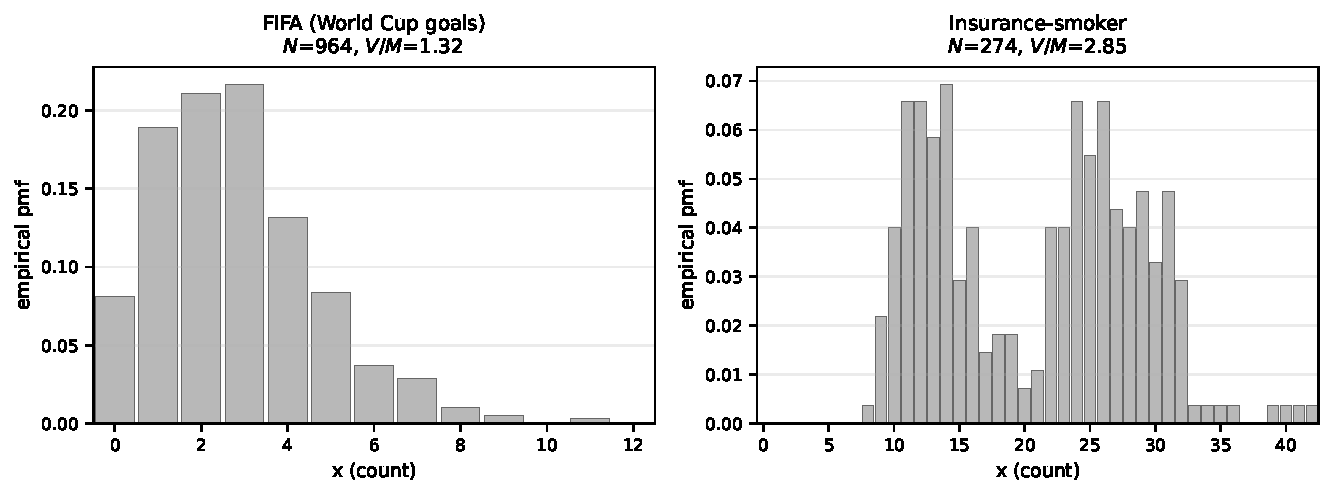
\includegraphics[width=0.85\textwidth]{data_pmf_overview_real.pdf}
\caption{Empirical pmfs of the two real datasets.}
\label{sfig:overview-real}
\end{figure}

\begin{figure}[H]\centering
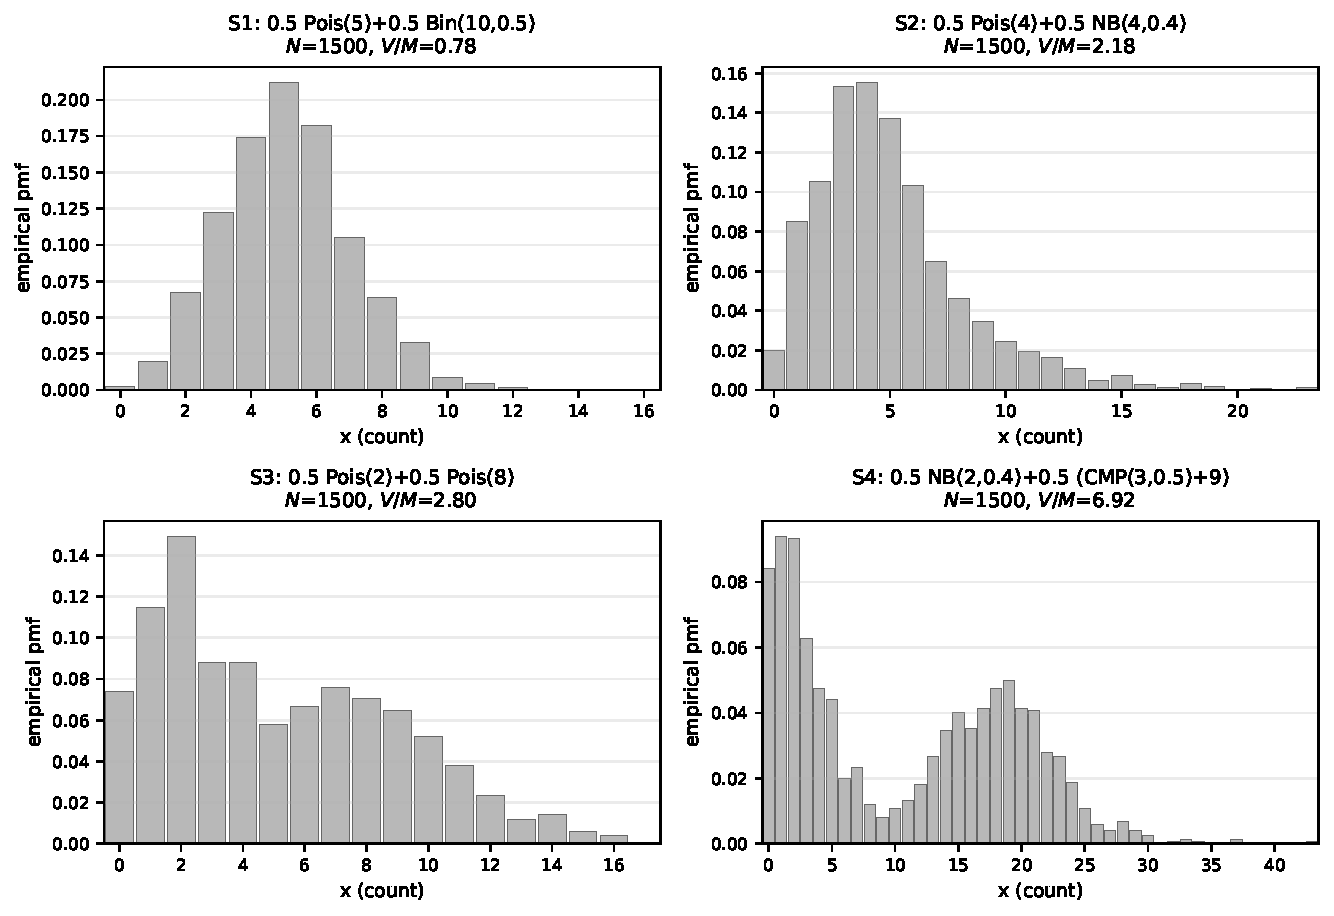
\includegraphics[width=0.85\textwidth]{data_pmf_overview_sim.pdf}
\caption{Empirical pmfs of the four simulation scenarios (fixed-seed samples, $N=1500$).}
\label{sfig:overview-sim}
\end{figure}

\section{Order-by-order goodness of fit, all datasets and estimators}

Tables~\ref{tab:l2-fifa}--\ref{tab:l2-s4} report the in-sample $L^1$ and unweighted
$L^2$ discrepancies of the three estimators (MoM, Sequential MLE, Joint MLE) at
every order of the comparison grid $K\in\{0,4,6,8,10,12,14\}$; the $K=4$ rows
coincide with the main text's fixed-order comparison, and the MoM column at
$K\in\{4,10,14\}$ coincides with the main text's cross-model table.

% Auto-generated by experiments/l2_eval.py
\begin{table}[H]
\centering
\caption{FIFA: in-sample $L^1$ and unweighted $L^2$ by truncation order $K$ for the three estimators (MoM/Seq/Joint).}
\label{tab:l2-fifa}
\small
\begin{tabular}{rrrrrrr}
\toprule
$K$ & \multicolumn{3}{c}{$L^1$} & \multicolumn{3}{c}{unweighted $L^2$} \\
\cmidrule(lr){2-4}\cmidrule(lr){5-7}
 & MoM & Seq & Joint & MoM & Seq & Joint \\
\midrule
0 & 0.0862 & 0.0844 & 0.0844 & 0.0349 & 0.0322 & 0.0322 \\
4 & 0.0674 & 0.0701 & 0.0679 & 0.0278 & 0.0277 & 0.0274 \\
6 & 0.0715 & 0.0705 & 0.0693 & 0.0271 & 0.0276 & 0.0272 \\
8 & 0.0674 & 0.0699 & 0.0685 & 0.0269 & 0.0273 & 0.0272 \\
10 & 0.0570 & 0.0433 & 0.0403 & 0.0214 & 0.0162 & 0.0154 \\
12 & 0.0316 & 0.0445 & 0.0409 & 0.0141 & 0.0168 & 0.0163 \\
14 & 0.0397 & 0.0319 & 0.0240 & 0.0166 & 0.0101 & 0.0084 \\
\bottomrule
\end{tabular}
\end{table}

% Auto-generated by experiments/l2_eval.py
\begin{table}[H]
\centering
\caption{Insurance-smoker: in-sample $L^1$ and unweighted $L^2$ by truncation order $K$ for the three estimators (MoM/Seq/Joint).}
\label{tab:l2-insurance_smoker}
\small
\begin{tabular}{rrrrrrr}
\toprule
$K$ & \multicolumn{3}{c}{$L^1$} & \multicolumn{3}{c}{unweighted $L^2$} \\
\cmidrule(lr){2-4}\cmidrule(lr){5-7}
 & MoM & Seq & Joint & MoM & Seq & Joint \\
\midrule
0 & 0.6115 & 0.6114 & 0.6114 & 0.1253 & 0.1252 & 0.1252 \\
4 & 0.6033 & 0.6001 & 0.5998 & 0.1235 & 0.1228 & 0.1234 \\
6 & 0.5353 & 0.5351 & 0.5271 & 0.1111 & 0.1110 & 0.1103 \\
8 & 0.4092 & 0.3766 & 0.3831 & 0.0865 & 0.0810 & 0.0835 \\
10 & 0.3569 & 0.3486 & 0.3431 & 0.0730 & 0.0722 & 0.0740 \\
12 & 0.2516 & 0.2476 & 0.2508 & 0.0526 & 0.0518 & 0.0526 \\
14 & 0.2478 & 0.2409 & 0.2409 & 0.0517 & 0.0536 & 0.0536 \\
\bottomrule
\end{tabular}
\end{table}

% Auto-generated by experiments/l2_eval.py
\begin{table}[H]
\centering
\caption{S1: in-sample $L^1$ and unweighted $L^2$ by truncation order $K$ for the three estimators (MoM/Seq/Joint).}
\label{tab:l2-s1}
\small
\begin{tabular}{rrrrrrr}
\toprule
$K$ & \multicolumn{3}{c}{$L^1$} & \multicolumn{3}{c}{unweighted $L^2$} \\
\cmidrule(lr){2-4}\cmidrule(lr){5-7}
 & MoM & Seq & Joint & MoM & Seq & Joint \\
\midrule
0 & 0.0748 & 0.0748 & 0.0748 & 0.0287 & 0.0287 & 0.0287 \\
4 & 0.0559 & 0.0547 & 0.0537 & 0.0193 & 0.0197 & 0.0196 \\
6 & 0.0589 & 0.0561 & 0.0557 & 0.0223 & 0.0212 & 0.0211 \\
8 & 0.0500 & 0.0471 & 0.0470 & 0.0183 & 0.0169 & 0.0169 \\
10 & 0.0293 & 0.0307 & 0.0307 & 0.0104 & 0.0112 & 0.0112 \\
12 & 0.0303 & 0.0320 & 0.0322 & 0.0111 & 0.0113 & 0.0113 \\
14 & 0.0297 & 0.0228 & 0.0228 & 0.0109 & 0.0087 & 0.0087 \\
\bottomrule
\end{tabular}
\end{table}

% Auto-generated by experiments/l2_eval.py
\begin{table}[H]
\centering
\caption{S2: in-sample $L^1$ and unweighted $L^2$ by truncation order $K$ for the three estimators (MoM/Seq/Joint).}
\label{tab:l2-s2}
\small
\begin{tabular}{rrrrrrr}
\toprule
$K$ & \multicolumn{3}{c}{$L^1$} & \multicolumn{3}{c}{unweighted $L^2$} \\
\cmidrule(lr){2-4}\cmidrule(lr){5-7}
 & MoM & Seq & Joint & MoM & Seq & Joint \\
\midrule
0 & 0.1974 & 0.1812 & 0.1812 & 0.0651 & 0.0567 & 0.0567 \\
4 & 0.0938 & 0.0882 & 0.0886 & 0.0273 & 0.0284 & 0.0265 \\
6 & 0.0836 & 0.0733 & 0.0752 & 0.0270 & 0.0266 & 0.0260 \\
8 & 0.0734 & 0.0702 & 0.0727 & 0.0257 & 0.0266 & 0.0261 \\
10 & 0.0629 & 0.0683 & 0.0515 & 0.0210 & 0.0209 & 0.0180 \\
12 & 0.0491 & 0.0620 & 0.0465 & 0.0155 & 0.0182 & 0.0133 \\
14 & 0.0411 & 0.0569 & 0.0404 & 0.0120 & 0.0171 & 0.0118 \\
\bottomrule
\end{tabular}
\end{table}

% Auto-generated by experiments/l2_eval.py
\begin{table}[H]
\centering
\caption{S3: in-sample $L^1$ and unweighted $L^2$ by truncation order $K$ for the three estimators (MoM/Seq/Joint).}
\label{tab:l2-s3}
\small
\begin{tabular}{rrrrrrr}
\toprule
$K$ & \multicolumn{3}{c}{$L^1$} & \multicolumn{3}{c}{unweighted $L^2$} \\
\cmidrule(lr){2-4}\cmidrule(lr){5-7}
 & MoM & Seq & Joint & MoM & Seq & Joint \\
\midrule
0 & 0.2400 & 0.2348 & 0.2348 & 0.0774 & 0.0735 & 0.0735 \\
4 & 0.1885 & 0.1836 & 0.1817 & 0.0672 & 0.0674 & 0.0679 \\
6 & 0.1838 & 0.1798 & 0.1800 & 0.0629 & 0.0602 & 0.0610 \\
8 & 0.1000 & 0.1033 & 0.1032 & 0.0341 & 0.0348 & 0.0346 \\
10 & 0.0991 & 0.0970 & 0.0963 & 0.0338 & 0.0336 & 0.0332 \\
12 & 0.0852 & 0.0805 & 0.0800 & 0.0311 & 0.0297 & 0.0297 \\
14 & 0.0767 & 0.0784 & 0.0773 & 0.0288 & 0.0284 & 0.0285 \\
\bottomrule
\end{tabular}
\end{table}

% Auto-generated by experiments/l2_eval.py
\begin{table}[H]
\centering
\caption{S4: in-sample $L^1$ and unweighted $L^2$ by truncation order $K$ for the three estimators (MoM/Seq/Joint).}
\label{tab:l2-s4}
\small
\begin{tabular}{rrrrrrr}
\toprule
$K$ & \multicolumn{3}{c}{$L^1$} & \multicolumn{3}{c}{unweighted $L^2$} \\
\cmidrule(lr){2-4}\cmidrule(lr){5-7}
 & MoM & Seq & Joint & MoM & Seq & Joint \\
\midrule
0 & 0.5852 & 0.5523 & 0.5523 & 0.1259 & 0.1137 & 0.1137 \\
4 & 0.4811 & 0.4834 & 0.4797 & 0.1030 & 0.0995 & 0.1022 \\
6 & 0.3335 & 0.3454 & 0.3147 & 0.0720 & 0.0768 & 0.0670 \\
8 & 0.2947 & 0.3002 & 0.3002 & 0.0636 & 0.0651 & 0.0651 \\
10 & 0.1621 & 0.1592 & 0.1540 & 0.0336 & 0.0347 & 0.0331 \\
12 & 0.1521 & 0.1403 & 0.1353 & 0.0319 & 0.0311 & 0.0293 \\
14 & 0.1350 & 0.1382 & 0.1160 & 0.0290 & 0.0312 & 0.0260 \\
\bottomrule
\end{tabular}
\end{table}


\section{PMF overlays: baselines versus CPOE by order (MoM)}

Each panel overlays the empirical pmf with the moment-matched baselines
(Poisson, NB, COM-Poisson) and the CPOE expansion at $K=4$, $10$, and $14$ (MoM).
The FIFA, Insurance-smoker, and S4 panels also appear in the main text and are
repeated here for completeness.

\begin{figure}[H]\centering
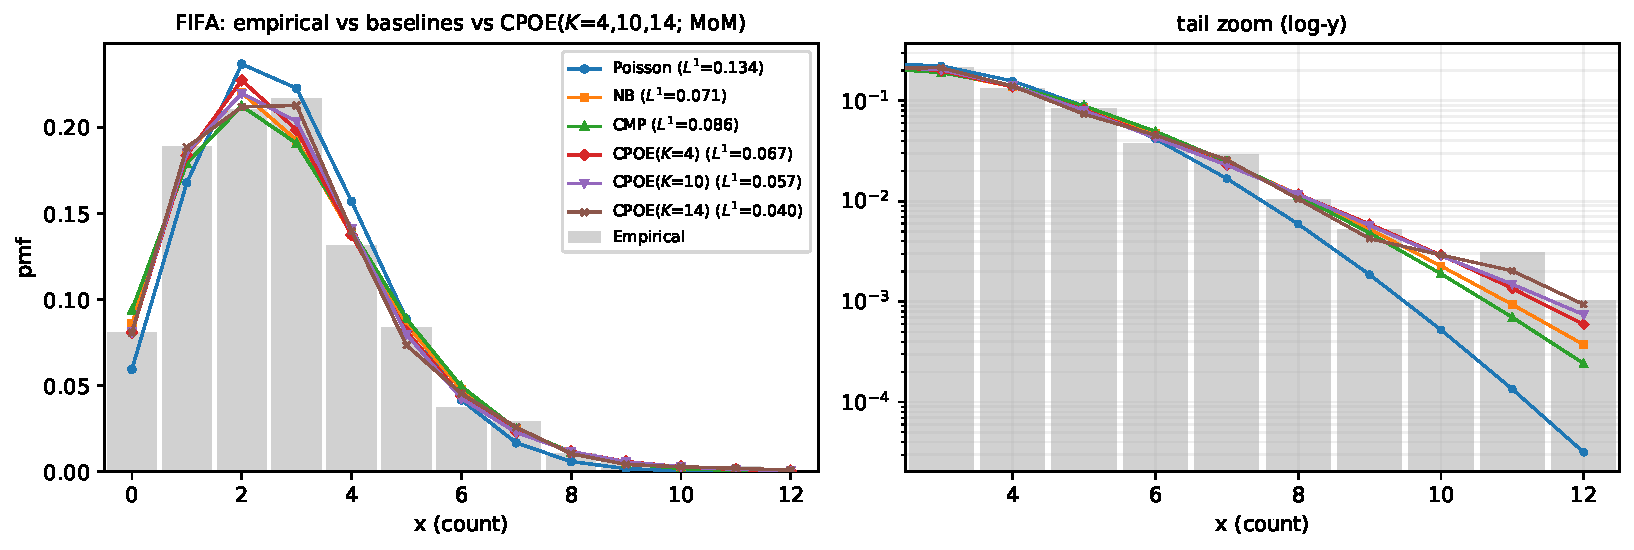
\includegraphics[width=\textwidth]{highk_pmfbase_fifa.pdf}
\caption{FIFA: empirical pmf versus baselines and CPOE at $K=4,10,14$ (MoM).}
\end{figure}
\begin{figure}[H]\centering
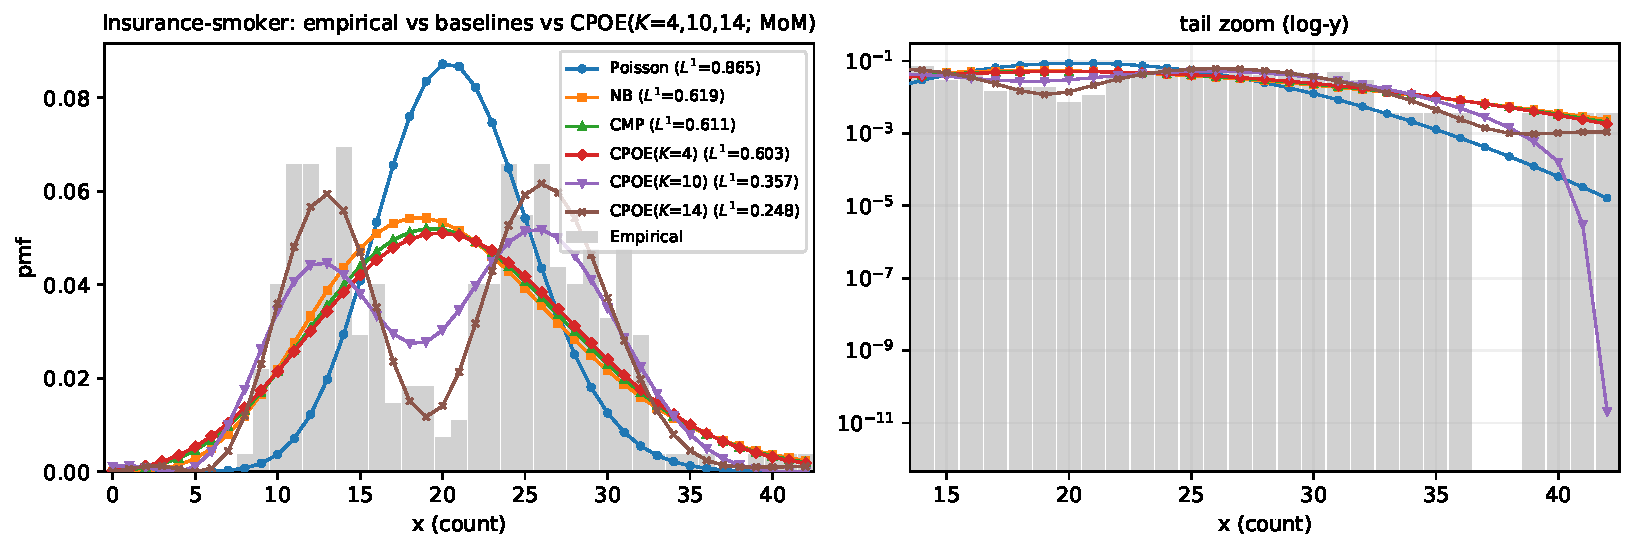
\includegraphics[width=\textwidth]{highk_pmfbase_insurance_smoker.pdf}
\caption{Insurance-smoker: empirical pmf versus baselines and CPOE at $K=4,10,14$ (MoM).}
\end{figure}
\begin{figure}[H]\centering
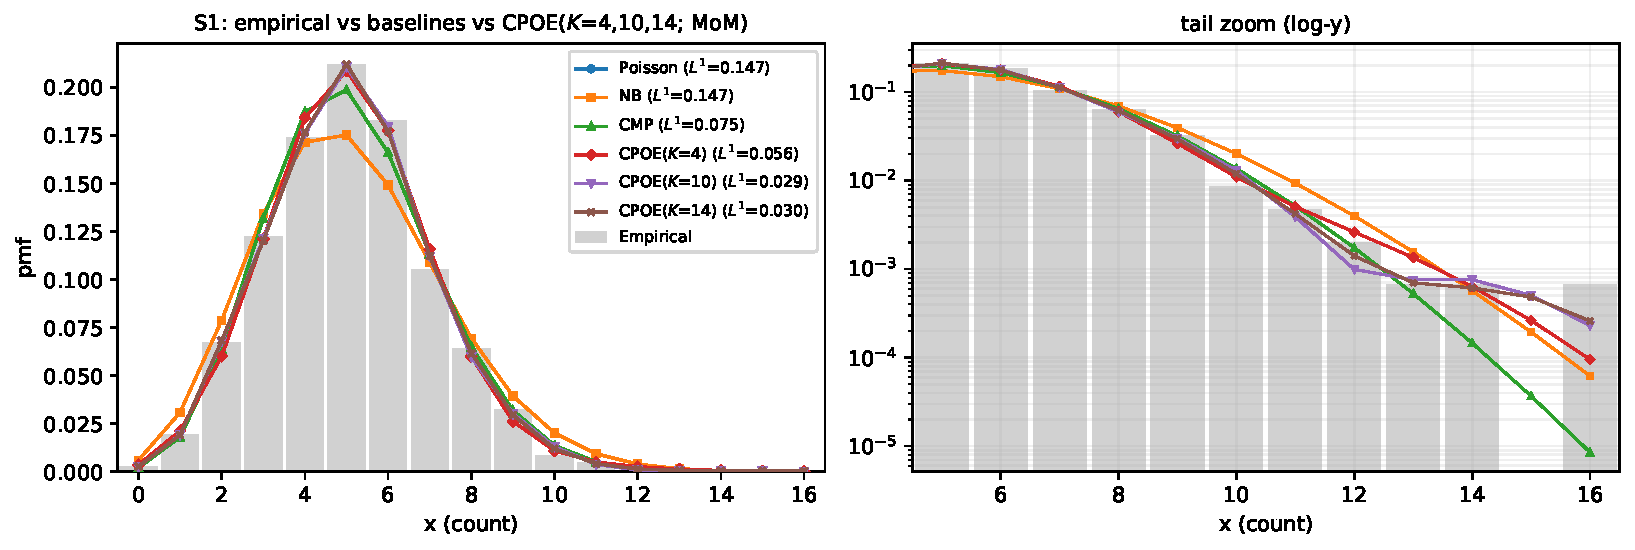
\includegraphics[width=\textwidth]{highk_pmfbase_s1.pdf}
\caption{S1: empirical pmf versus baselines and CPOE at $K=4,10,14$ (MoM).}
\end{figure}
\begin{figure}[H]\centering
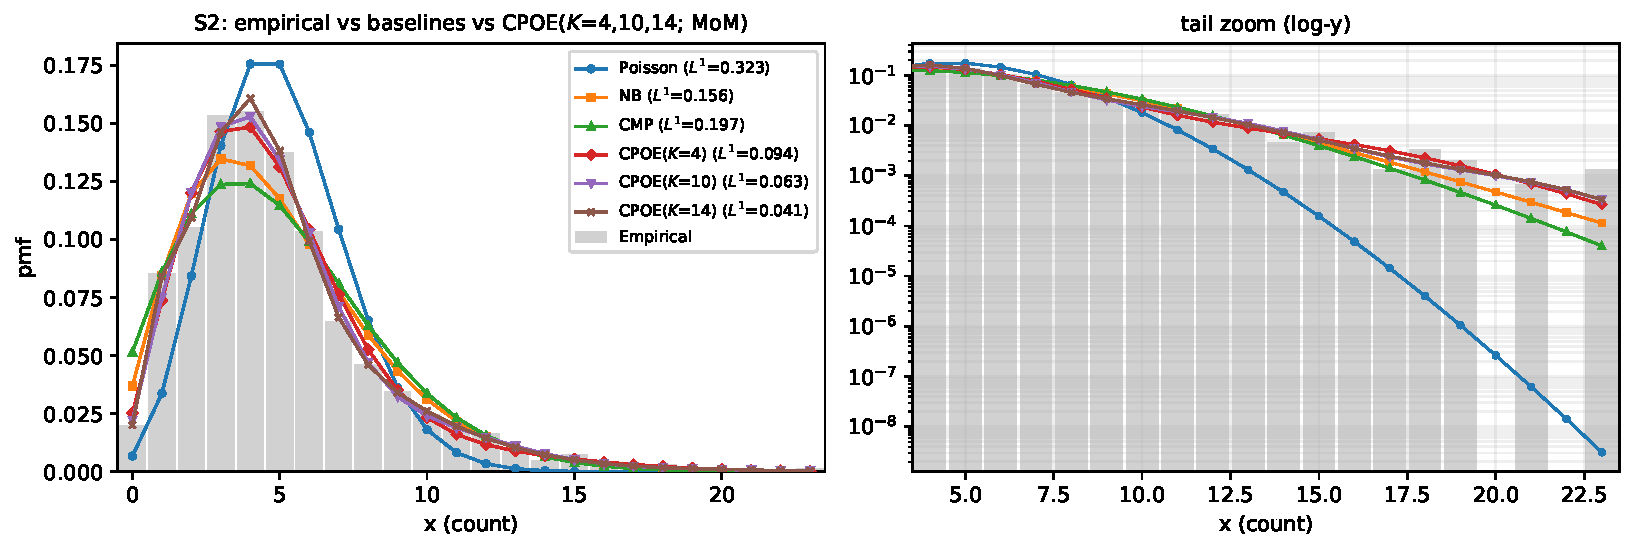
\includegraphics[width=\textwidth]{highk_pmfbase_s2.pdf}
\caption{S2: empirical pmf versus baselines and CPOE at $K=4,10,14$ (MoM).}
\end{figure}
\begin{figure}[H]\centering
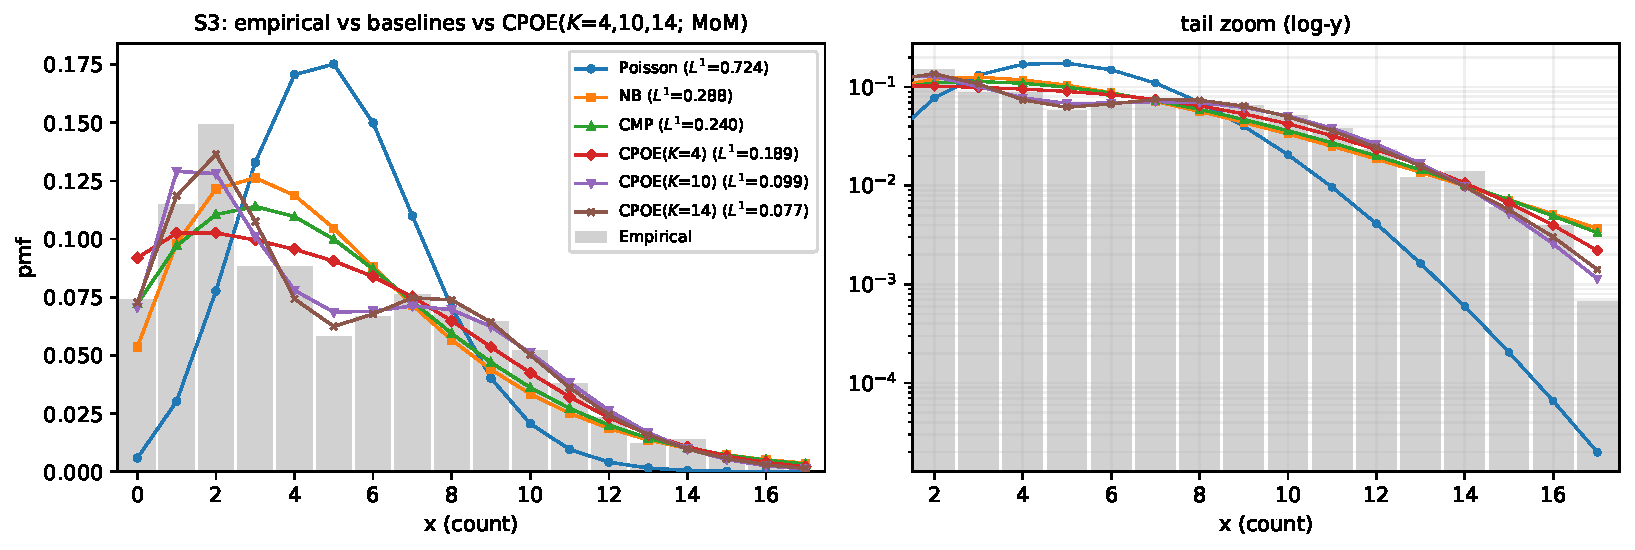
\includegraphics[width=\textwidth]{highk_pmfbase_s3.pdf}
\caption{S3: empirical pmf versus baselines and CPOE at $K=4,10,14$ (MoM).}
\end{figure}
\begin{figure}[H]\centering
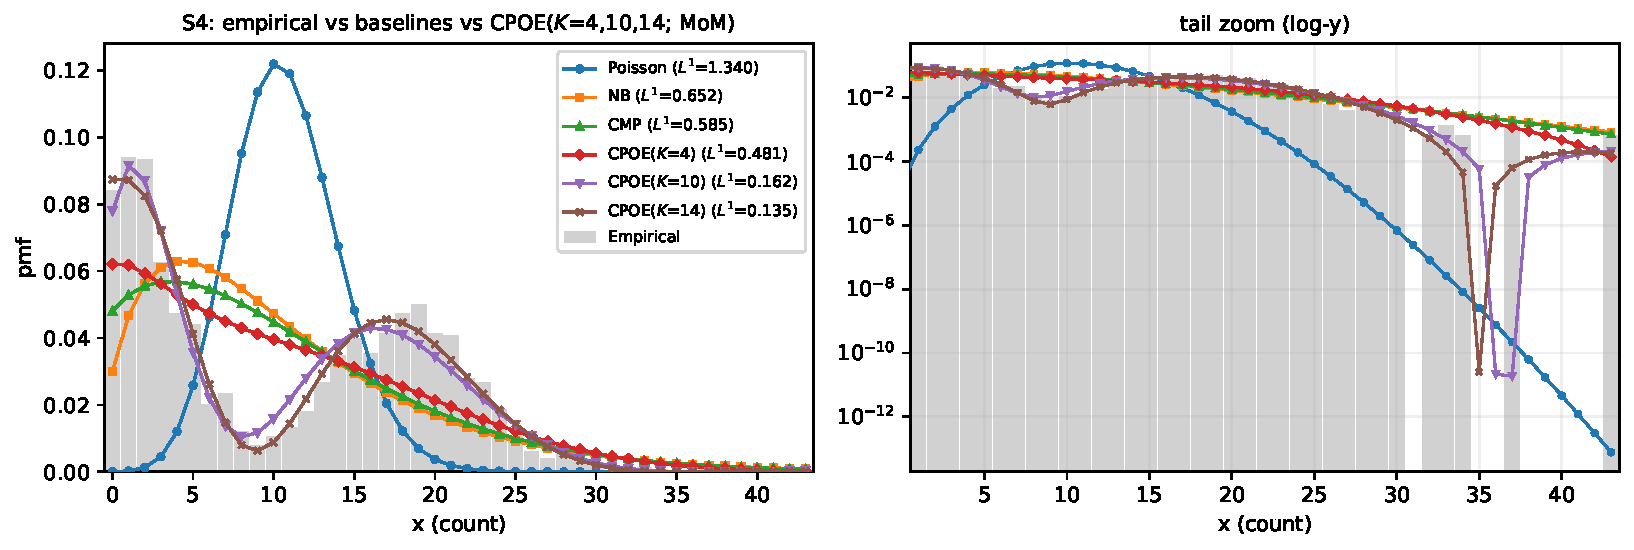
\includegraphics[width=\textwidth]{highk_pmfbase_s4.pdf}
\caption{S4: empirical pmf versus baselines and CPOE at $K=4,10,14$ (MoM).}
\end{figure}

\section{Same-order overlays of the three estimators}

The following overlays compare the fitted CPOE pmfs of the three estimators at the
common orders $K=10$ and $K=14$; the near-coincidence of the three curves is the
estimator-equivalence phenomenon discussed in the main text.

\begin{figure}[H]\centering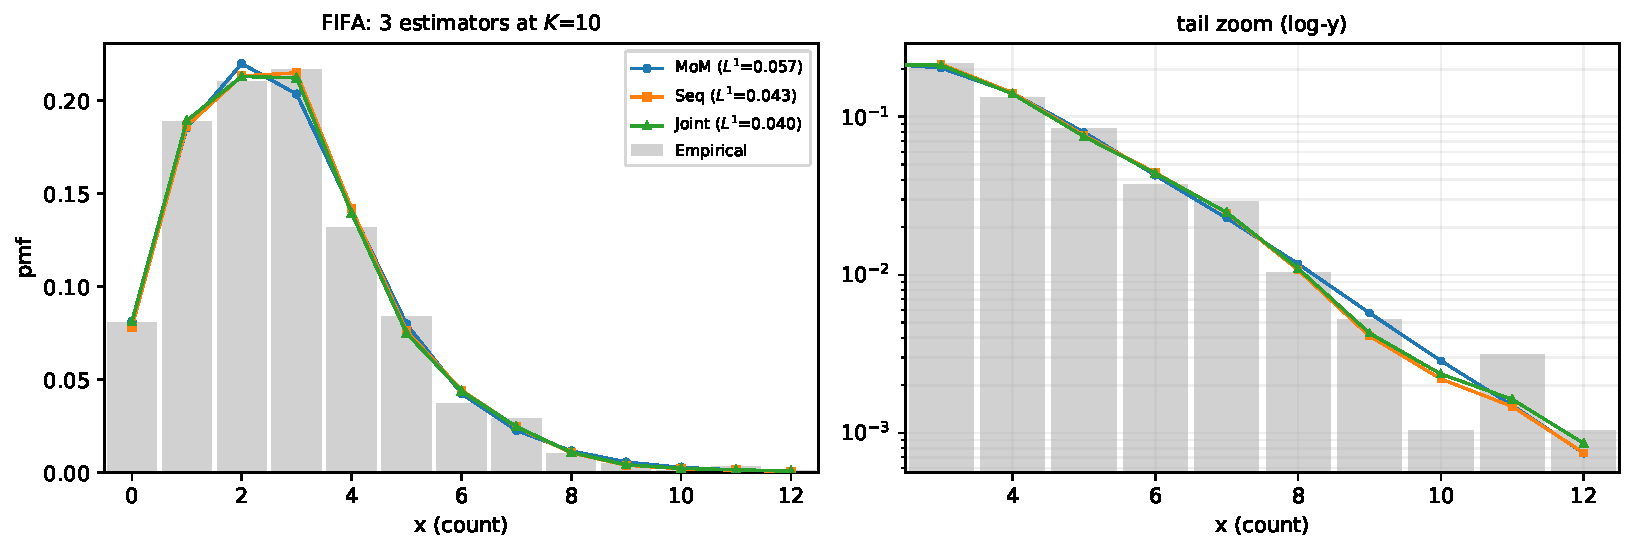
\includegraphics[width=\textwidth]{highk_estpmf_fifa_K10.pdf}\caption{FIFA: empirical pmf versus the CPOE pmfs of the three estimators at the same order $K{=}10$. Left: linear scale; right: tail on a logarithmic $y$-axis.}\label{fig:hk-fifa-estpmf-k10}\end{figure}
\begin{figure}[H]\centering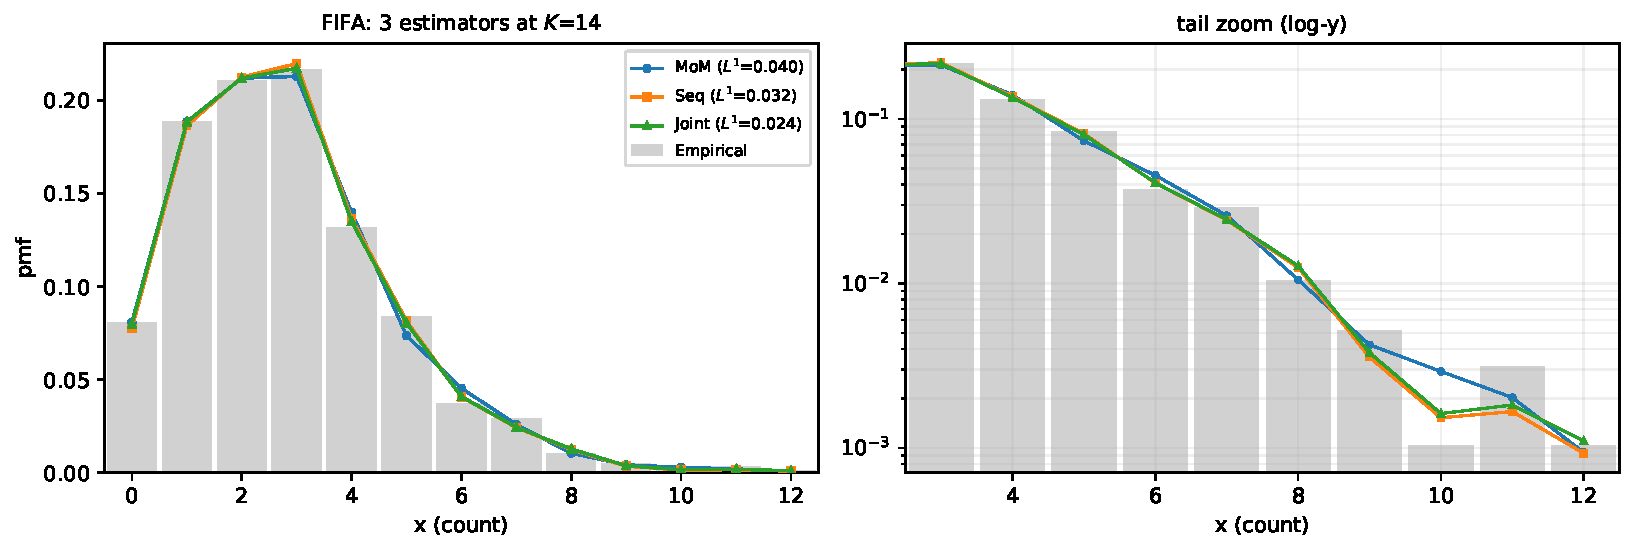
\includegraphics[width=\textwidth]{highk_estpmf_fifa_K14.pdf}\caption{FIFA: empirical pmf versus the CPOE pmfs of the three estimators at the same order $K{=}14$. Left: linear scale; right: tail on a logarithmic $y$-axis.}\label{fig:hk-fifa-estpmf-k14}\end{figure}

\begin{figure}[H]\centering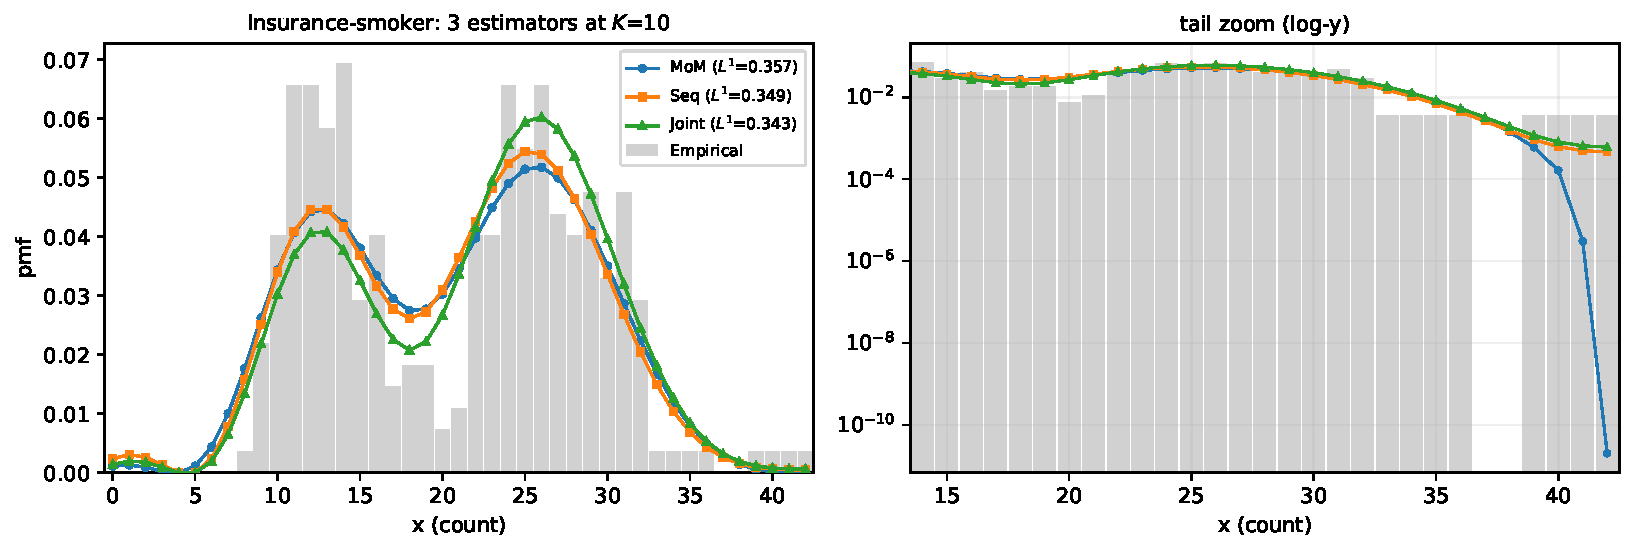
\includegraphics[width=\textwidth]{highk_estpmf_insurance_smoker_K10.pdf}\caption{Insurance-smoker: empirical pmf versus the CPOE pmfs of the three estimators at the same order $K{=}10$. Left: linear scale; right: tail on a logarithmic $y$-axis.}\label{fig:hk-insurance_smoker-estpmf-k10}\end{figure}
\begin{figure}[H]\centering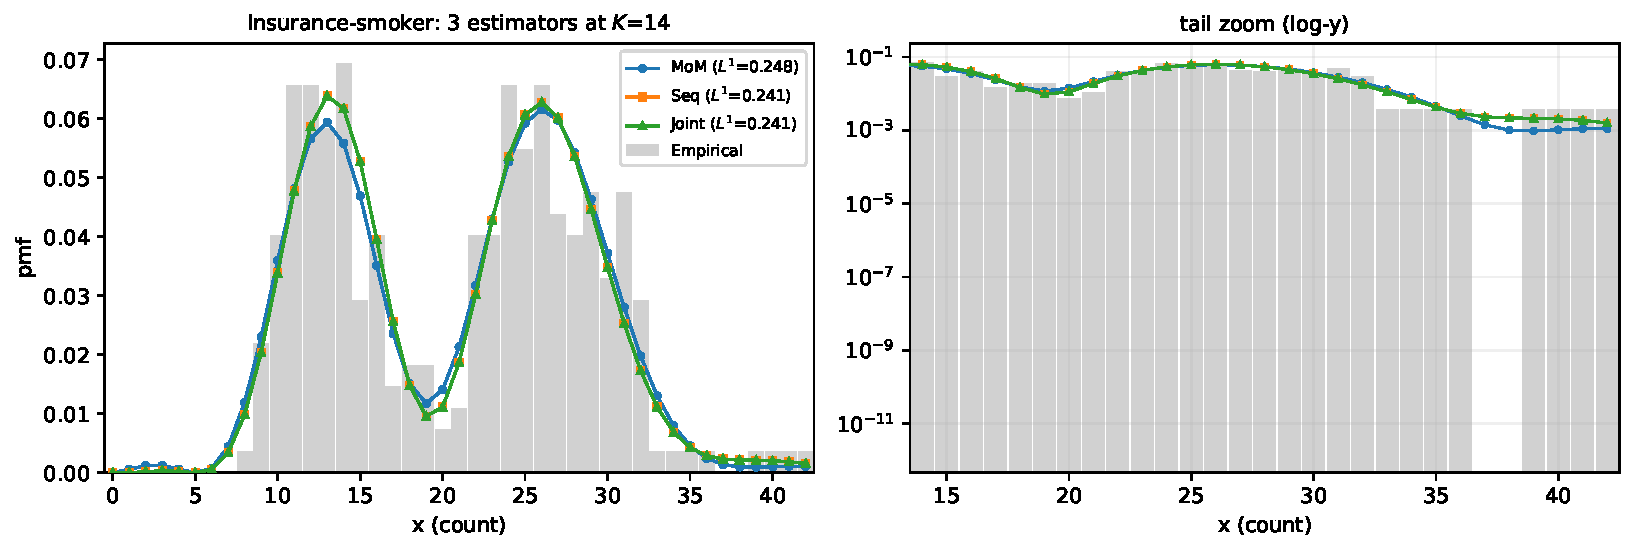
\includegraphics[width=\textwidth]{highk_estpmf_insurance_smoker_K14.pdf}\caption{Insurance-smoker: empirical pmf versus the CPOE pmfs of the three estimators at the same order $K{=}14$. Left: linear scale; right: tail on a logarithmic $y$-axis.}\label{fig:hk-insurance_smoker-estpmf-k14}\end{figure}

\input{tables/highk_estpmf_s1.tex}
\begin{figure}[H]\centering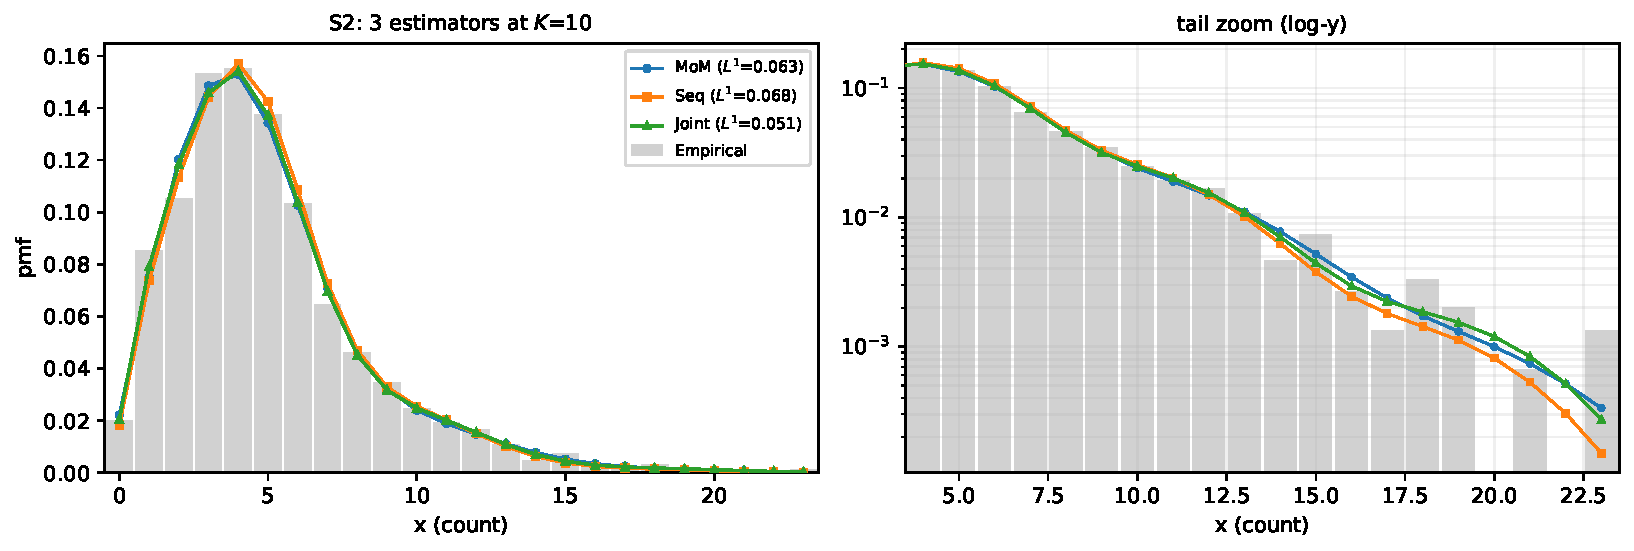
\includegraphics[width=\textwidth]{highk_estpmf_s2_K10.pdf}\caption{S2: empirical pmf versus the CPOE pmfs of the three estimators at the same order $K{=}10$. Left: linear scale; right: tail on a logarithmic $y$-axis.}\label{fig:hk-s2-estpmf-k10}\end{figure}
\begin{figure}[H]\centering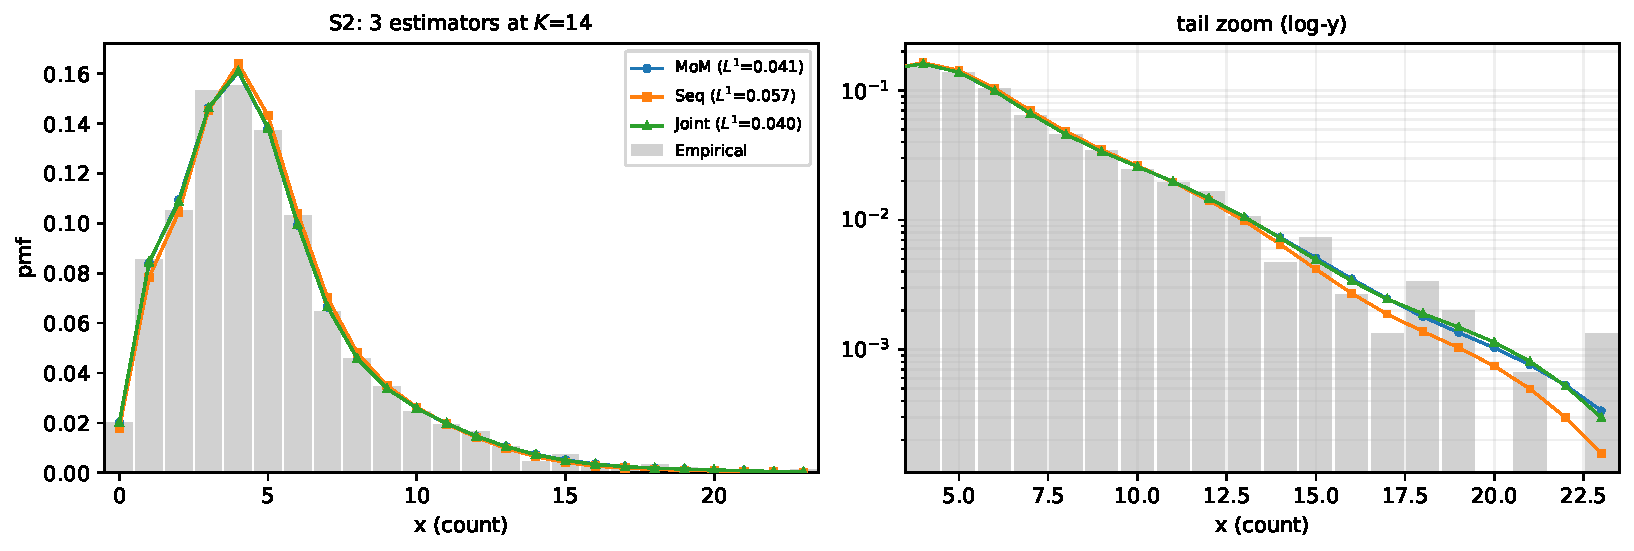
\includegraphics[width=\textwidth]{highk_estpmf_s2_K14.pdf}\caption{S2: empirical pmf versus the CPOE pmfs of the three estimators at the same order $K{=}14$. Left: linear scale; right: tail on a logarithmic $y$-axis.}\label{fig:hk-s2-estpmf-k14}\end{figure}

\begin{figure}[H]\centering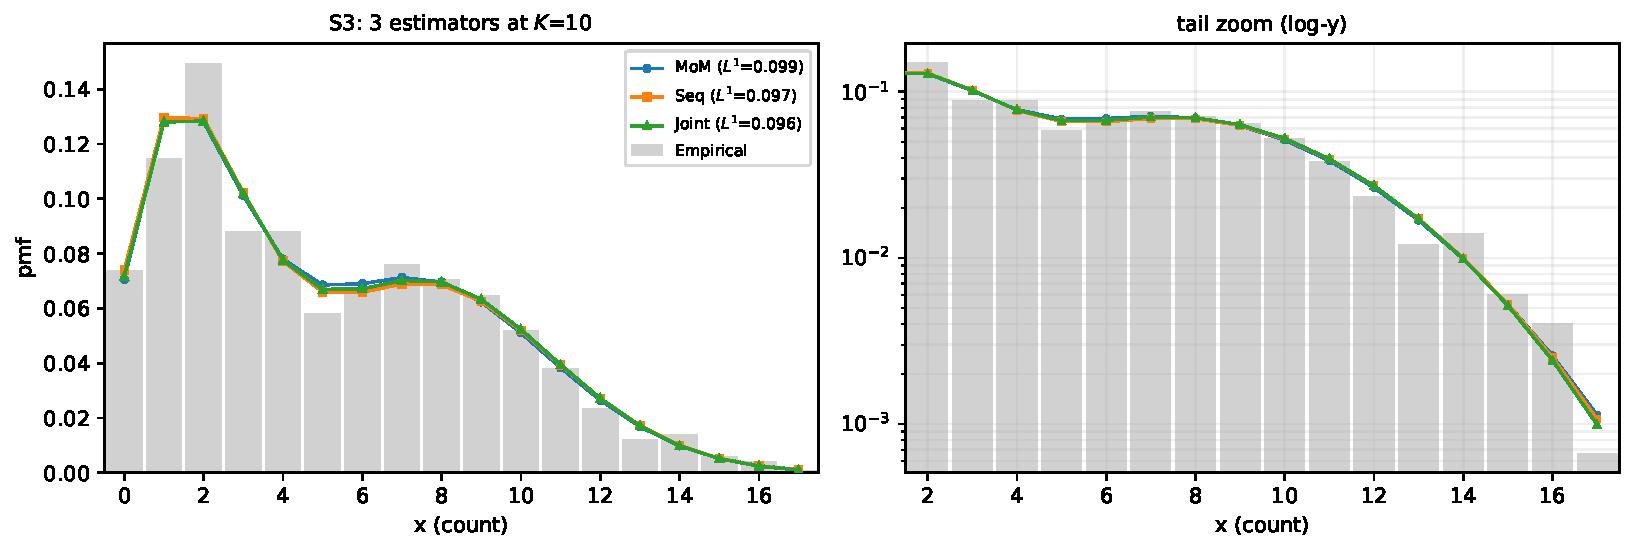
\includegraphics[width=\textwidth]{highk_estpmf_s3_K10.pdf}\caption{S3: empirical pmf versus the CPOE pmfs of the three estimators at the same order $K{=}10$. Left: linear scale; right: tail on a logarithmic $y$-axis.}\label{fig:hk-s3-estpmf-k10}\end{figure}
\begin{figure}[H]\centering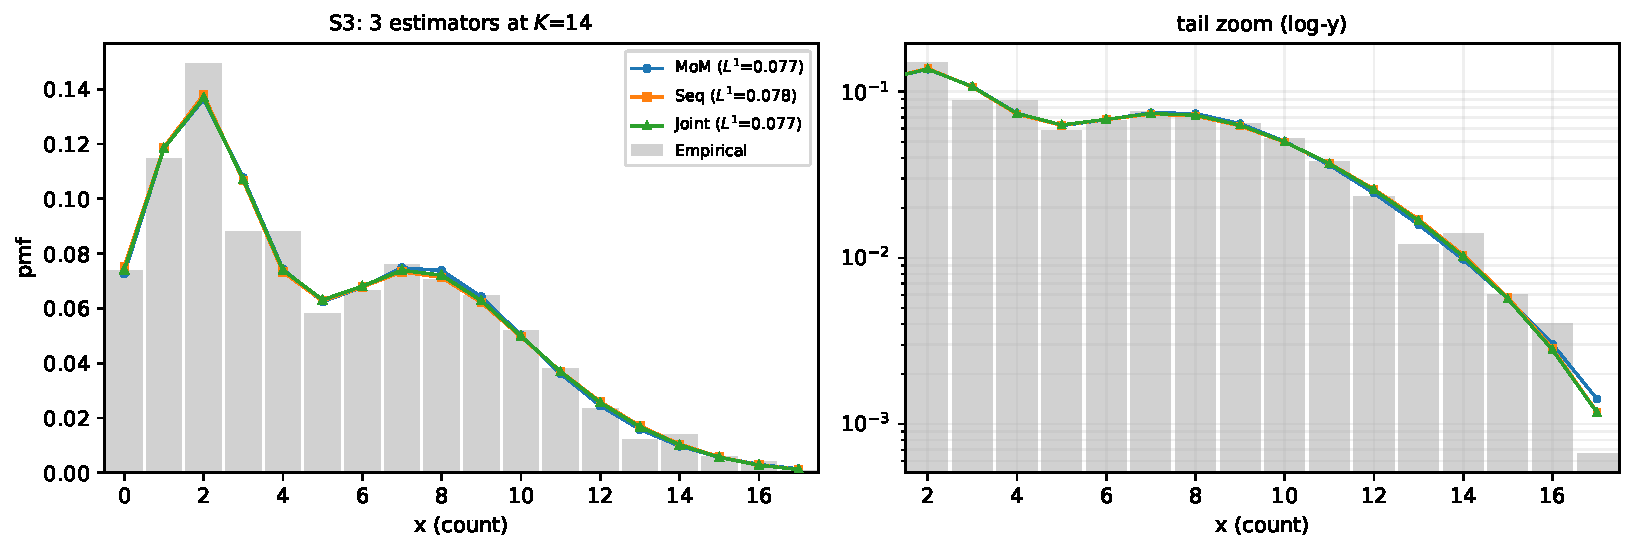
\includegraphics[width=\textwidth]{highk_estpmf_s3_K14.pdf}\caption{S3: empirical pmf versus the CPOE pmfs of the three estimators at the same order $K{=}14$. Left: linear scale; right: tail on a logarithmic $y$-axis.}\label{fig:hk-s3-estpmf-k14}\end{figure}

\begin{figure}[H]\centering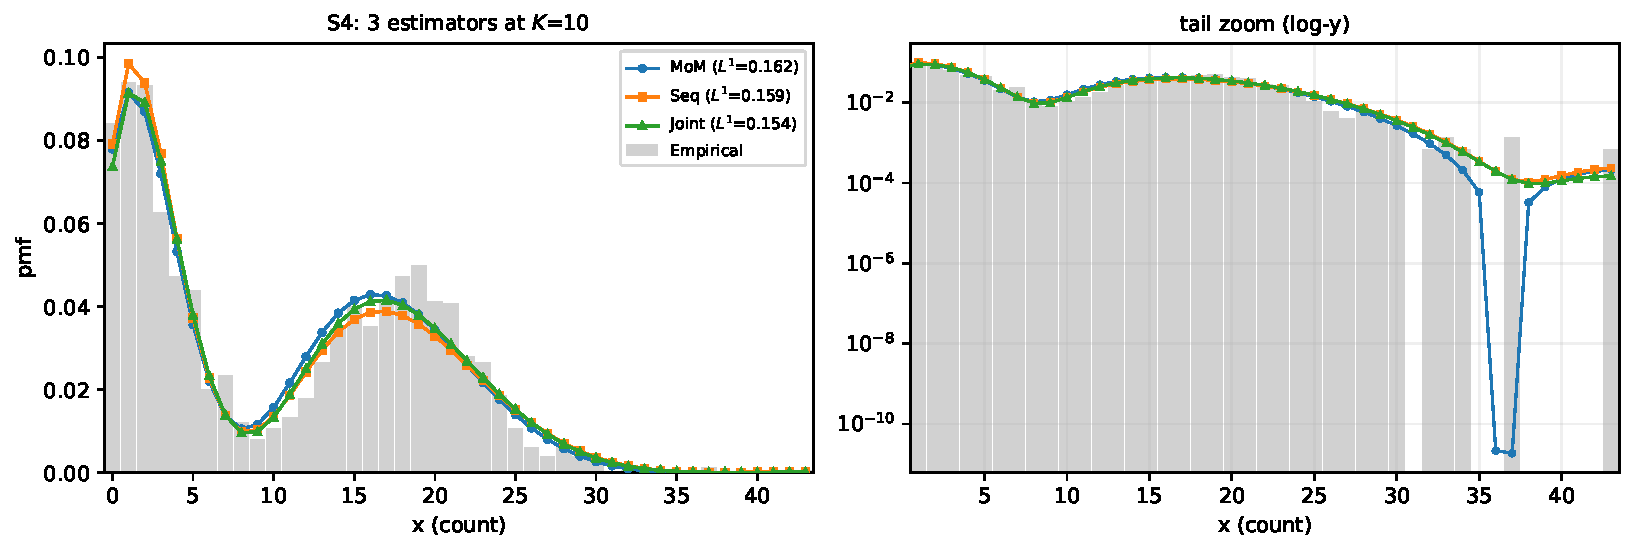
\includegraphics[width=\textwidth]{highk_estpmf_s4_K10.pdf}\caption{S4: empirical pmf versus the CPOE pmfs of the three estimators at the same order $K{=}10$. Left: linear scale; right: tail on a logarithmic $y$-axis.}\label{fig:hk-s4-estpmf-k10}\end{figure}
\begin{figure}[H]\centering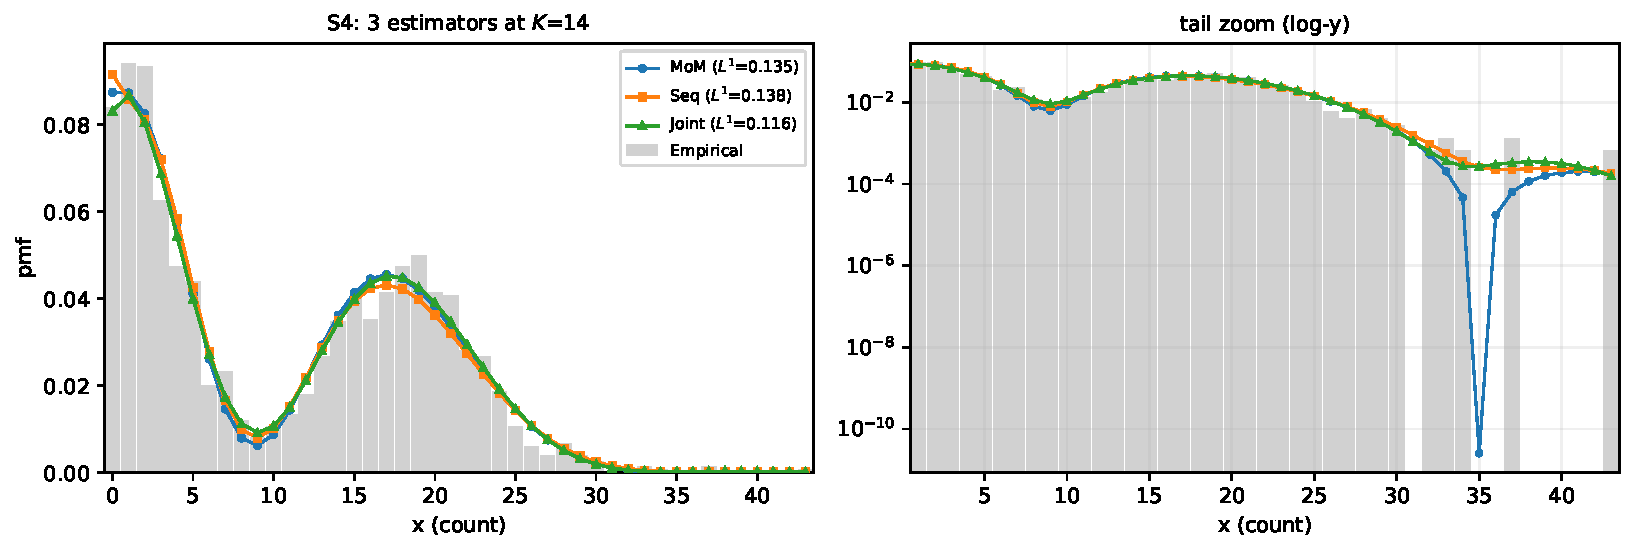
\includegraphics[width=\textwidth]{highk_estpmf_s4_K14.pdf}\caption{S4: empirical pmf versus the CPOE pmfs of the three estimators at the same order $K{=}14$. Left: linear scale; right: tail on a logarithmic $y$-axis.}\label{fig:hk-s4-estpmf-k14}\end{figure}


\section{Numerical construction of the orthonormal basis}

This section backs the main text's quantitative claims on the finite-precision
behavior of the two basis constructions (Hankel/Cholesky versus the three-term
recurrence obtained by a discretized-Stieltjes procedure).

% Auto-generated by experiments/task1_basis_comparison.py
\begin{table}[H]
\centering
\caption{Comparison of the two numerical constructions of the orthonormal basis (Hankel/Cholesky vs three-term recurrence/Stieltjes) on three synthetic $(\lambda,\nu)$ combinations and degrees $n\in\{1,2,3,4,9\}$. $E_\perp=\max_{i,j}|\langle\psi_i,\psi_j\rangle-\delta_{ij}|$ is the orthonormality error, $\Delta_{\mathrm{coef}}$ the maximum coefficient difference between the two methods, mem the peak memory (KB), and $t$ the median computation time (ms). The two methods agree at low degree, but at $n=9$ the ill-conditioning of the Hankel matrix degrades the Cholesky orthonormality to $\sim$$10^{-6}$ while the three-term recurrence maintains $\sim$$10^{-12}$ (Gautschi 2004).}
\label{tab:task1-basis}
\footnotesize
\begin{tabular}{llrrrrrrr}
\toprule
Dispersion & $n$ & $E_\perp^{\mathrm{Ch}}$ & $E_\perp^{\mathrm{TTR}}$ & $\Delta_{\mathrm{coef}}$ & mem$_{\mathrm{Ch}}$ & mem$_{\mathrm{TTR}}$ & $t_{\mathrm{Ch}}$ & $t_{\mathrm{TTR}}$ \\
\midrule
\multirow{5}{*}{under-dispersed} & 1 & $1.0\mathrm{e}-15$ & $1.0\mathrm{e}-15$ & $4.4\mathrm{e}-16$ & 7.6 & 2.4 & 0.126 & 0.022 \\
 & 2 & $5.4\mathrm{e}-14$ & $1.3\mathrm{e}-15$ & $1.7\mathrm{e}-13$ & 7.9 & 2.9 & 0.120 & 0.040 \\
 & 3 & $1.2\mathrm{e}-12$ & $3.6\mathrm{e}-15$ & $5.1\mathrm{e}-12$ & 8.4 & 3.2 & 0.137 & 0.058 \\
 & 4 & $1.1\mathrm{e}-12$ & $1.7\mathrm{e}-14$ & $8.8\mathrm{e}-12$ & 8.9 & 3.5 & 0.173 & 0.079 \\
 & 9 & $1.2\mathrm{e}-06$ & $1.3\mathrm{e}-12$ & $3.9\mathrm{e}-05$ & 12.8 & 5.1 & 0.315 & 0.217 \\
\midrule
\multirow{5}{*}{near-equidispersed} & 1 & $4.2\mathrm{e}-15$ & $1.1\mathrm{e}-15$ & $7.1\mathrm{e}-15$ & 7.8 & 2.8 & 0.110 & 0.021 \\
 & 2 & $1.1\mathrm{e}-14$ & $1.1\mathrm{e}-15$ & $2.8\mathrm{e}-14$ & 8.2 & 3.4 & 0.143 & 0.039 \\
 & 3 & $3.4\mathrm{e}-14$ & $3.6\mathrm{e}-15$ & $2.3\mathrm{e}-13$ & 8.7 & 3.8 & 0.155 & 0.058 \\
 & 4 & $9.9\mathrm{e}-13$ & $1.6\mathrm{e}-14$ & $2.3\mathrm{e}-12$ & 9.3 & 4.1 & 0.169 & 0.079 \\
 & 9 & $1.0\mathrm{e}-06$ & $5.4\mathrm{e}-13$ & $1.7\mathrm{e}-05$ & 13.5 & 6.0 & 0.316 & 0.218 \\
\midrule
\multirow{5}{*}{over-dispersed} & 1 & $4.2\mathrm{e}-15$ & $8.5\mathrm{e}-16$ & $6.2\mathrm{e}-15$ & 9.2 & 5.4 & 0.113 & 0.022 \\
 & 2 & $3.9\mathrm{e}-14$ & $1.2\mathrm{e}-15$ & $1.1\mathrm{e}-13$ & 10.0 & 6.3 & 0.134 & 0.041 \\
 & 3 & $1.1\mathrm{e}-12$ & $4.9\mathrm{e}-15$ & $5.5\mathrm{e}-12$ & 11.1 & 7.1 & 0.155 & 0.059 \\
 & 4 & $9.2\mathrm{e}-12$ & $1.2\mathrm{e}-14$ & $6.0\mathrm{e}-11$ & 13.2 & 7.8 & 0.182 & 0.082 \\
 & 9 & $1.5\mathrm{e}-06$ & $7.9\mathrm{e}-12$ & $2.7\mathrm{e}-05$ & 24.1 & 11.5 & 0.323 & 0.223 \\
\bottomrule
\end{tabular}
\end{table}


\begin{figure}[H]\centering
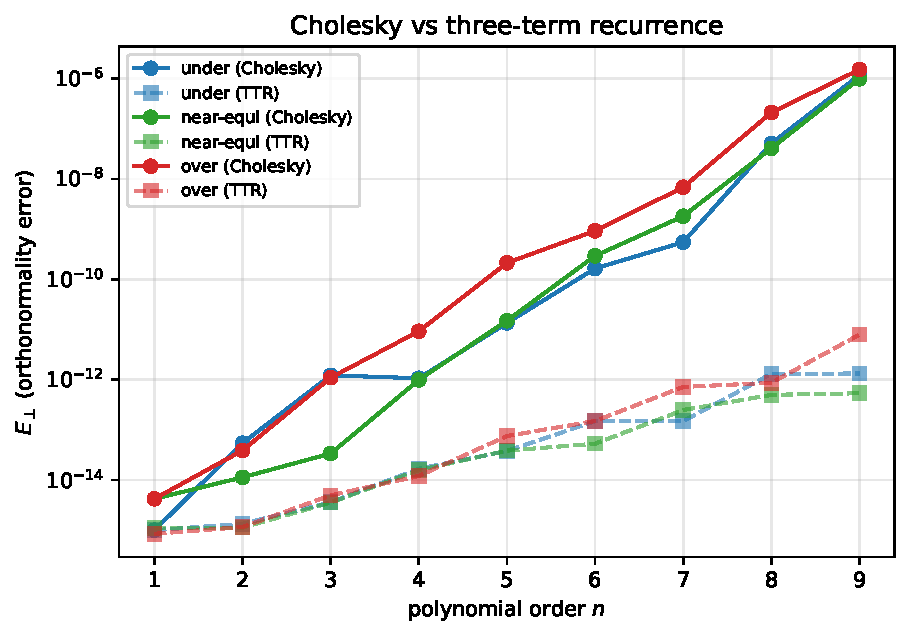
\includegraphics[width=0.8\textwidth]{task1_conditioning.pdf}
\caption{Orthonormality error versus degree for the Hankel/Cholesky construction
(solid) and the three-term recurrence (dashed) on the three synthetic
$(\lambda,\nu)$ combinations.}
\label{sfig:task1-cond}
\end{figure}

Explicit low-order polynomials $\psi_1,\ldots,\psi_4$ at the three synthetic
$(\lambda,\nu)$ combinations (three-term-recurrence coefficients):

% Auto-generated by experiments/task1_basis_comparison.py
% Given (lambda, nu), each psi_n is an explicit polynomial in x.
\paragraph{Under-dispersed $(\lambda=10,\nu=1.5)$}
\begin{align*}
  \psi_1(x) &= -2.5383 + 0.5680x \\
  \psi_2(x) &= 4.5235 - 2.1894x + 0.2280x^{2} \\
  \psi_3(x) &= -6.5140 + 5.1735x - 1.1499x^{2} + 0.0747x^{3} \\
  \psi_4(x) &= 8.0010 - 9.4154x + 3.3727x^{2} - 0.4626x^{3} + 0.0212x^{4} \\
\end{align*}
\paragraph{Near-equidispersed $(\lambda=5,\nu=0.95)$}
\begin{align*}
  \psi_1(x) &= -2.2856 + 0.4179x \\
  \psi_2(x) &= 3.6984 - 1.4809x + 0.1235x^{2} \\
  \psi_3(x) &= -4.8952 + 3.2585x - 0.5831x^{2} + 0.0298x^{3} \\
  \psi_4(x) &= 5.6243 - 5.6163x + 1.6254x^{2} - 0.1756x^{3} + 0.0062x^{4} \\
\end{align*}
\paragraph{Over-dispersed $(\lambda=3,\nu=0.4)$}
\begin{align*}
  \psi_1(x) &= -2.6223 + 0.1603x \\
  \psi_2(x) &= 4.9043 - 0.6405x + 0.0182x^{2} \\
  \psi_3(x) &= -7.5760 + 1.5926x - 0.0954x^{2} + 0.0017x^{3} \\
  \psi_4(x) &= 10.2883 - 3.1092x + 0.2951x^{2} - 0.0109x^{3} + 0.0001x^{4} \\
\end{align*}


\end{document}
